% =====================================================================
% HammerTime - Half-Way (50%) Project Report  (expanded edition)
% Compiles on Overleaf with pdfLaTeX (default). No BibTeX needed.
% Required image files (put in an assets/ folder):
%   assets/graph_snapshot.png   (was core_graph_visualization.png)
%   assets/analytics.png        (was core_analytics.png)
%   assets/terminal_run.jpg     (was Photo_from_andromeda____2_.jpg)
% =====================================================================
\documentclass[11pt,a4paper]{article}

\usepackage[utf8]{inputenc}
\usepackage[T1]{fontenc}
\usepackage{mathpazo}
\usepackage[a4paper,margin=1in]{geometry}
\usepackage{graphicx}
\graphicspath{{assets/}}
\usepackage{amsmath,amssymb}
\usepackage{booktabs}
\usepackage{tabularx}
\usepackage{array}
\usepackage{multirow}
\usepackage{longtable}
\usepackage[table]{xcolor}
\usepackage{caption}
\usepackage{subcaption}
\usepackage{float}
\usepackage{enumitem}
\usepackage{listings}
\usepackage{fancyhdr}
\usepackage{setspace}
\usepackage{algorithm}
\usepackage{algpseudocode}
\usepackage[most]{tcolorbox}
\usepackage{tikz}
\usetikzlibrary{positioning,arrows.meta,shapes.geometric,fit,calc,decorations.pathreplacing}
\usepackage{pgfplots}
\pgfplotsset{compat=1.16}
\usepackage[colorlinks=true,linkcolor=blue!50!black,citecolor=blue!50!black,urlcolor=blue!50!black]{hyperref}

\setstretch{1.12}
\captionsetup{font=small,labelfont=bf}
\setlist{itemsep=2pt,topsep=4pt}

% ---------------- Author placeholders (edit these) -------------------
\newcommand{\authorAname}{A. Adithya Sai Pratheek}
\newcommand{\authorAreg}{24BAI1445}
\newcommand{\authorBname}{M.S. Abhinav Sriram}
\newcommand{\authorBreg}{24BAI1209}
\newcommand{\affil}{SCOPE -- VIT Chennai}

% ---------------- Colours -------------------------------------------
\definecolor{f1red}{HTML}{E10600}
\definecolor{f1orange}{HTML}{FF9900}
\definecolor{f1green}{HTML}{10B981}
\definecolor{carbon}{HTML}{15151E}

% ---------------- Call-out boxes ------------------------------------
\newtcolorbox{keybox}[1]{colback=blue!4,colframe=blue!50!black,fonttitle=\bfseries\small,
  title=#1,boxrule=0.6pt,arc=2pt,left=6pt,right=6pt,top=4pt,bottom=4pt}
\newtcolorbox{warnbox}[1]{colback=red!4,colframe=red!60!black,fonttitle=\bfseries\small,
  title=#1,boxrule=0.6pt,arc=2pt,left=6pt,right=6pt,top=4pt,bottom=4pt}

% ---------------- Listings ------------------------------------------
\lstset{
  basicstyle=\ttfamily\footnotesize,
  breaklines=true,
  frame=single,
  backgroundcolor=\color{gray!8},
  rulecolor=\color{gray!50},
  columns=fullflexible,
  keepspaces=true,
  language=Python,
  keywordstyle=\color{blue!60!black}\bfseries,
  commentstyle=\color{green!40!black}\itshape,
  stringstyle=\color{red!50!black}
}

% ---------------- Header / footer -----------------------------------
\pagestyle{fancy}
\fancyhf{}
\lhead{\small HammerTime -- Project Report}
\rhead{\small \affil}
\cfoot{\thepage}
\renewcommand{\headrulewidth}{0.4pt}

\newcommand{\dt}{\Delta t}
\algrenewcommand\algorithmicrequire{\textbf{Input:}}
\algrenewcommand\algorithmicensure{\textbf{Output:}}

\begin{document}

% =====================================================================
% TITLE PAGE
% =====================================================================
\begin{titlepage}
\centering
\vspace*{1.2cm}
{\large \textsc{BCSE209L -- Machine Learning}\par}
{\large \textsc{Vellore Institute of Technology, Chennai}\par}
\vspace{1.6cm}
\rule{\linewidth}{1.2pt}\\[0.5cm]
{\Huge \bfseries HammerTime\par}
\vspace{0.3cm}
{\Large A Dynamic Spatio-Temporal Graph Neural Network\\for Formula~1 Traffic Delay Estimation\par}
\vspace{0.3cm}
\rule{\linewidth}{1.2pt}\\[1.0cm]
{\Large \textbf{Project Report (50\% Core Implementation)}\par}
\vspace{0.4cm}
{\large Case study: 2021 Abu Dhabi Grand Prix\par}
\vspace{2.2cm}

\begin{tabularx}{\linewidth}{XX}
\centering \textbf{\large \authorAname} & \centering \textbf{\large \authorBname} \tabularnewline[4pt]
\centering \authorAreg & \centering \authorBreg \tabularnewline[4pt]
\centering \affil & \centering \affil \tabularnewline
\end{tabularx}

\vfill
{\large \today}
\end{titlepage}

% =====================================================================
% ABSTRACT
% =====================================================================
\begin{abstract}
In Formula~1, a car that follows closely behind another loses downforce and
tyre performance because it drives in the leader's turbulent wake (``dirty
air''). This loss is rarely measured directly. HammerTime is a project that
estimates it as a per-car, per-mini-sector time delay $\Delta t_{\text{sector}}$
with a dynamic spatio-temporal graph neural network (ST-GNN). This report
describes the work completed at the half-way point.

The 50\% core implementation ingests real telemetry of the 2021 Abu Dhabi
Grand Prix through the FastF1 library (416{,}879 aligned rows, 19 drivers),
resamples it to a 4~Hz grid, computes the time gap between consecutive cars,
and builds 21{,}941 graph snapshots with 137{,}355 directed
leader-to-follower edges weighted by a Gaussian radial basis function (RBF).
A lightweight message-passing network (3{,}393 trainable parameters) with
temporal pooling is trained on 4{,}112 windows and evaluated on the final
1{,}371 windows of the race. The data pipeline, the graph builder, the graph
visualiser, the training loop and the analytics module all run end to end.

The prediction accuracy does not yet meet the targets: on the held-out
windows the model reaches an MAE of 1.14~s and an $R^2$ of 0.29, against
targets of $<0.15$~s and 0.68--0.82. This report gives these numbers without
adjustment and analyses their causes. Code inspection shows that the target
look-up used for training is not lap-aware, which means that the current
test figures are a preliminary baseline and not a valid estimate of
generalisation. The report also covers the Safety Car period of the race,
target clipping, label quantisation and the single-hop design of the model,
and it sets out a concrete, testable plan for the second half of the project.

\medskip
\noindent\textbf{Keywords:} Formula~1, graph neural network, spatio-temporal
learning, dirty air, FastF1, message passing, traffic delay, motorsport
analytics.
\end{abstract}

\newpage
\tableofcontents
\newpage
\listoffigures
\listoftables
\newpage

% =====================================================================
\section{Introduction}
% =====================================================================

\subsection{Background: Aerodynamics and Racing in Traffic}
A Formula~1 car produces a large part of its grip from aerodynamic downforce.
The front wing, floor, diffuser and rear wing shape the air around the car, and
the air that leaves the car is turbulent and slower than the free stream. A
second car that drives close behind meets this disturbed air. The follower
then produces less downforce, especially at the front axle. Corner speed
falls, the car slides more, and the tyres run hotter. The effect is strongest
in fast corners and decreases as the gap grows.

This effect has two consequences for race strategy. First, a faster car often
cannot pass a slower one, because the follower loses the pace it needs to
close up through the corners. Second, a car that stays in traffic wears its
tyres faster than a car in clean air, so the lap time loss is not limited to
the lap on which it is measured. The Drag Reduction System (DRS) lets a
follower within one second of the car ahead open a rear-wing flap on
designated straights, but it does not remove the loss in the corners. A group
of cars that all run within DRS range of each other is called a \emph{DRS
train}. In such a train the cars move at the pace of the slowest car, and
passing becomes very hard.

\subsection{Why the 2021 Abu Dhabi Grand Prix}
The 2021 Abu Dhabi Grand Prix is a convenient case study for three reasons.
It is the last race of the season, so the data is complete and well documented.
It has a full field with many close battles, including the lead
fight between M.~Verstappen (\texttt{VER}) and L.~Hamilton (\texttt{HAM}).
It also contains a Safety Car period from lap~53, after the crash of
N.~Latifi, which makes it a hard test case: the final laps of the race do not
follow the normal racing physics that the model is meant to learn. The
project uses this fact as a diagnostic (see Section~\ref{sec:analysis}).

\subsection{Motivation}
Teams know the dirty-air effect qualitatively, but broadcast graphics and
public timing screens show only the gap in seconds. They do not show how much
lap time the follower actually loses. A model that estimates this
\emph{traffic delay} for every car at every place on the circuit would help in
three ways:
\begin{itemize}[leftmargin=*]
  \item it would explain \emph{why} a faster car cannot pass, with a number;
  \item it would give strategists a cost for staying in traffic, which
        supports pit-stop decisions;
  \item it would give broadcasters a clear visual story (who is slowing whom).
\end{itemize}

\subsection{Problem Statement and Formalisation}
A race is a sequence of states of the whole field. Let
$\mathcal{V}=\{1,\dots,N\}$ be the set of cars ($N=19$ in the data used here)
and let $t \in \{0, \Delta\tau, 2\Delta\tau, \dots\}$ be discrete time with
$\Delta\tau = 0.25$~s. At each time step, the field is a directed graph
\begin{equation}
\mathcal{G}_t = (\mathcal{V}, \mathcal{E}_t, \mathbf{X}_t, \mathbf{e}_t),
\end{equation}
where $\mathbf{X}_t \in \mathbb{R}^{N\times F}$ holds the node features,
$\mathcal{E}_t$ is the set of directed leader-to-follower edges and
$\mathbf{e}_t$ holds the edge weights. Given the last $W$ graphs,
\begin{equation}
\hat{\mathbf{y}}_{t+h} = f_\theta\bigl(\mathcal{G}_{t-W+1},\dots,\mathcal{G}_t\bigr), \qquad \hat{\mathbf{y}}\in\mathbb{R}^{N},
\end{equation}
the task is to predict for every car $i$ the extra time
\begin{equation}
\Delta t^{(i)}_{\text{sector}} = t^{(i)}_{\text{actual}} - t_{\text{clean-air}}
\end{equation}
that the car needs for the mini-sector it will be in at time $t+h$, compared
with the time that the same sector takes in clean air.

\subsection{Objectives}
\begin{enumerate}[leftmargin=*]
  \item Build a repeatable pipeline that turns raw race telemetry into an
        aligned time-series table that includes the gap to the car ahead.
  \item Represent the race as a sequence of directed graphs in which an edge
        means ``car $j$ disturbs car $i$'', with a physically motivated weight.
  \item Train a spatio-temporal GNN to predict $\Delta t_{\text{sector}}$.
  \item Visualise the disturbance graph and the traffic statistics in a form
        that is suitable for broadcast use.
  \item (Second half) Add attention, safety-car filtering, baselines and a
        physics validation suite, and reach the accuracy targets.
\end{enumerate}

\subsection{Work Completed in the First Half}
\begin{itemize}[leftmargin=*]
  \item A FastF1 ingestion and alignment module with a Parquet cache.
  \item A gap computation and clean-air target module.
  \item A dynamic graph builder (21{,}941 snapshots; 137{,}355 edges).
  \item A tiered, broadcast-style graph visualiser with an adjacency matrix.
  \item A trainable message-passing ST-GNN with a masked loss and a
        chronological train/test protocol.
  \item An analytics module (DRS-train detector, parity plot, histogram).
  \item A command-line runner with three modes (\texttt{full}, \texttt{graph},
        \texttt{train}).
  \item A critical review of the results, with a list of confirmed and
        suspected problems and a plan to fix them.
\end{itemize}

\subsection{Organisation of this Report}
Section~\ref{sec:background} reviews related work. Section~\ref{sec:design}
states the requirements and the main design decisions. Sections~\ref{sec:data}
to~\ref{sec:model} describe the data, the graph and the model. Section~\ref{sec:setup}
gives the experimental protocol, Section~\ref{sec:results} the results, and
Section~\ref{sec:analysis} the analysis and limitations. Sections~\ref{sec:vv} to
\ref{sec:future} cover verification, project management and the plan for
the second half. Section~\ref{sec:conclusion} concludes.

\subsection{Notation}
\begin{table}[H]
\centering
\caption{Notation used in this report.}
\label{tab:notation}
\small
\begin{tabularx}{\linewidth}{@{}lX@{}}
\toprule
\textbf{Symbol} & \textbf{Meaning} \\
\midrule
$N$, $\mathcal{V}$ & Number of cars (nodes) and the set of cars \\
$\Delta\tau$ & Sampling interval ($0.25$~s at 4~Hz) \\
$\dt_{ij}$ & Time gap (s) between leader $j$ and follower $i$ \\
$e_{ij}$ & Edge weight (Gaussian RBF of the gap) \\
$\sigma$ & Kernel width ($1.0$~s) \\
$\mathbf{x}_i \in \mathbb{R}^{F}$ & Node feature vector ($F=4$ in the core model) \\
$\mathbf{h}_i \in \mathbb{R}^{D}$ & Hidden state of car $i$ ($D=32$) \\
$W$, $K$ & Window length and prediction offset (both 5 snapshots) \\
$S$ & Number of mini-sectors per lap ($20$) \\
$\Delta t_{\text{sector}}$ & Target: sector time minus clean-air baseline \\
$m_i$ & Mask: 1 if car $i$ has a label in the sample, else 0 \\
\bottomrule
\end{tabularx}
\end{table}

% =====================================================================
\section{Background and Related Work}
\label{sec:background}
% =====================================================================

\subsection{Graph Neural Networks}
Graph neural networks learn a representation of each node from its own
features and the features of its neighbours. The graph convolutional network
of Kipf and Welling \cite{kipf2017} averages neighbour features with fixed
weights from the graph structure. The message-passing framework of Gilmer
\emph{et al.}\ \cite{gilmer2017} generalises this: a \emph{message} is computed
on every edge from the states of the two end nodes and the edge features, the
messages that arrive at a node are \emph{aggregated} (for example by a sum),
and the node state is \emph{updated}. The model in this project follows this
pattern. Graph attention networks \cite{velickovic2018} let the network learn
how much each neighbour should contribute, and they will replace the fixed
sum in the 100\% version.

\subsection{Spatio-Temporal Graph Models}
Many problems have a graph structure that changes over time. Traffic
forecasting is the standard example: the nodes are road sensors and the
signals are speed or flow. Yu \emph{et al.}\ \cite{yu2018} combine graph
convolution with temporal convolution to predict traffic. The same idea
applies to a race. Here the ``road'' is the changing neighbourhood of cars
around the circuit, and the ``speed'' is the time lost in a sector.

\subsection{Position of this Work}
\begin{table}[H]
\centering
\caption{Qualitative comparison of modelling choices for traffic delay.}
\label{tab:related}
\small
\begin{tabularx}{\linewidth}{@{}lXXX@{}}
\toprule
\textbf{Approach} & \textbf{Uses other cars?} & \textbf{Edge information?} & \textbf{Handles time?} \\
\midrule
Single-car regression (e.g.\ gradient boosting) & Only as hand-made features (gap) & No & Via lag features \\
Single-car sequence model (LSTM) & Only as hand-made features & No & Yes \\
Graph convolution \cite{kipf2017} & Yes & Fixed structure & No \\
Graph attention \cite{velickovic2018} & Yes & Learned weights & No \\
ST-GNN (this project, core) & Yes & Weighted, directed (RBF) & Yes (pooling) \\
ST-GNN (this project, 100\%) & Yes & Weighted, directed + attention & Yes (temporal convolution) \\
\bottomrule
\end{tabularx}
\end{table}
The central idea is that the interaction between two cars is not a feature of
one car but a property of the pair. A graph keeps this pair information as an
explicit edge. The two baselines of the 100\% plan (isolated single-car
XGBoost and LSTM) will test whether this explicit structure improves the
prediction.

\subsection{Tools}
The FastF1 library gives access to official timing and telemetry data
\cite{fastf1}. PyTorch is used for the model \cite{paszke2019}, the Adam
optimiser for training \cite{kingma2015}, and scikit-learn for the regression
metrics \cite{pedregosa2011}.

% =====================================================================
\section{Requirements and Design Rationale}
\label{sec:design}
% =====================================================================

\subsection{Requirements}
\begin{table}[H]
\centering
\caption{Requirements of the core (50\%) implementation.}
\label{tab:requirements}
\small
\begin{tabularx}{\linewidth}{@{}llXl@{}}
\toprule
\textbf{ID} & \textbf{Type} & \textbf{Requirement} & \textbf{Status} \\
\midrule
R1 & Functional & Load real race telemetry and cache it locally & Met \\
R2 & Functional & Align all cars on a common time grid & Met \\
R3 & Functional & Compute the gap to the car ahead at each step & Met \\
R4 & Functional & Build a directed, weighted graph per time step & Met \\
R5 & Functional & Compute clean-air delay targets per mini-sector & Met (see \S\ref{sec:analysis}) \\
R6 & Functional & Train and evaluate a spatio-temporal GNN & Met \\
R7 & Functional & Visualise the graph and the traffic statistics & Met \\
R8 & Non-functional & Rebuild all graphs in about half a minute from cache & Met (about 25~s) \\
R9 & Non-functional & One command reproduces the full run & Met \\
\bottomrule
\end{tabularx}
\end{table}

\subsection{Design Decisions}
\begin{table}[H]
\centering
\caption{Main design decisions and their rationale.}
\label{tab:decisions}
\small
\begin{tabularx}{\linewidth}{@{}p{2.6cm}p{3.0cm}X@{}}
\toprule
\textbf{Decision} & \textbf{Alternative} & \textbf{Rationale} \\
\midrule
4~Hz common time grid & Native, irregular samples & One grid makes every snapshot a complete graph and keeps the memory small. 0.25~s is fine enough to follow gap changes and coarse enough to run on a laptop. \\
Directed edges leader$\to$follower & Undirected edges & Wake travels from the leader to the follower. A directed edge keeps the cause and the effect separate and lets the model learn an asymmetric influence. \\
Edge only to the car directly ahead & Edges to all cars within range & It keeps the graph sparse (about 6 edges per snapshot) and matches the physics: the car directly ahead produces the wake. Longer-range influence is left to multi-hop message passing. \\
Gaussian RBF weight & Binary edge; inverse gap $1/\dt$ & It is smooth, bounded in $(0,1]$, and has no singularity at small gaps. The width $\sigma$ has a clear meaning in seconds. \\
2~s edge limit & 1.0~s or 3.0~s & Beyond about 2~s the RBF weight is below 0.14. A 3~s limit would match the clean-air definition but would add many weak edges. \\
Clean-air baseline from the same race & Fixed reference lap & It adapts to track temperature, fuel and tyre state of this race. The price is that the baseline depends on the data. \\
Masked L1 loss & Mean squared error & L1 is less sensitive to the large outliers in the target (see Figure~\ref{fig:analytics}). A mask is needed because not every car has a label in every window. \\
Chronological split & Random split & A random split would mix neighbouring windows (which overlap in time) between train and test and would overstate performance. \\
Small model (3{,}393 parameters) & Large model & The 50\% goal is a fast, inspectable baseline. A small model also exposes problems in the data earlier. \\
\bottomrule
\end{tabularx}
\end{table}

\subsection{Two Fixed Rules}
The project fixes two rules in the specification. They are called ``laws''
in the project documents.
\begin{keybox}{Law 1 -- Edge rule}
A directed disturbance edge from the leader $j$ to the follower $i$ exists if
and only if $0 < \dt_{ij} \le 2.0$~s.
\end{keybox}
\begin{keybox}{Law 2 -- Clean-air target isolation}
The target is the \emph{excess} time over a clean-air baseline,
$\Delta t_{\text{sector}} = t_{\text{actual}} - \operatorname{median}(t_{\text{sector}} \mid \dt > 3.0\text{ s})$.
The model never receives a clean-air reference as an input feature.
\end{keybox}

% =====================================================================
\section{Data Ingestion and Preprocessing}
\label{sec:data}
% =====================================================================

\subsection{Source Data}
The race session of the 2021 Abu Dhabi Grand Prix (58 laps) is loaded with
FastF1. For each driver, the per-lap telemetry is concatenated and sorted by
time. The channels used are \emph{Speed}, \emph{Throttle} and
\emph{Distance}. The first call downloads the data. After that, the aligned
table is read from a Parquet file, which avoids repeated network access
(requirement R1).

\subsection{Schema of the Aligned Table}
\begin{table}[H]
\centering
\caption{Columns of the aligned telemetry table.}
\label{tab:schema}
\small
\begin{tabularx}{\linewidth}{@{}llX@{}}
\toprule
\textbf{Column} & \textbf{Type} & \textbf{Description} \\
\midrule
\texttt{TimeSec} & float & Session time in seconds, uniform grid with step 0.25 \\
\texttt{Driver} & str & Driver identifier (racing number as a string) \\
\texttt{Speed} & float & Speed in km/h, linearly interpolated \\
\texttt{Throttle} & float & Throttle position in percent, interpolated \\
\texttt{Distance} & float & Cumulative distance in metres, interpolated \\
\texttt{LapNumber} & int & Derived: $\lfloor d / L \rfloor + 1$ \\
\texttt{MiniSector} & int & Derived: sector index in $\{0,\dots,19\}$ \\
\texttt{Compound} & str & Constant \texttt{MEDIUM} in the core version (placeholder) \\
\texttt{TyreLife} & float & Set equal to the lap number in the core version \\
\texttt{IsPitLap} & bool & Constant \texttt{False} in the core version (placeholder) \\
\texttt{DriverAhead} & str & Driver directly ahead by distance, or \texttt{None} \\
\texttt{DeltaT} & float & Time gap to the car ahead in seconds ($99$ if none) \\
\bottomrule
\end{tabularx}
\end{table}

\subsection{Temporal Alignment}
The telemetry of each car is sampled at its own irregular time stamps. Every
channel is linearly interpolated onto one common grid with
$f_s = 4$~Hz ($\Delta\tau = 0.25$~s). The grid starts at the earliest and
ends at the latest time stamp found over all cars. The aligned table has
416{,}879 rows for 19 drivers, that is, $21{,}941$ time steps per driver
($416{,}879 / 19 = 21{,}941$ exactly). At 4~Hz this is about 91.4 minutes of
session time.

\subsection{Mini-Sectors and Lap Counter}
The circuit is divided into $S = 20$ equal mini-sectors. With lap length
$L = 5281$~m, each mini-sector is $L/S = 264.05$~m long. For a car at
cumulative distance $d$,
\begin{equation}
s = \min\!\left(\left\lfloor \frac{(d \bmod L)}{L/S} \right\rfloor,\, S-1\right), \qquad
\text{lap} = \left\lfloor \frac{d}{L} \right\rfloor + 1.
\end{equation}

\subsection{Gap to the Car Ahead}
Algorithm~\ref{alg:gap} computes the gap at one time step. The cars are sorted
by cumulative distance. For the follower $i$ and the car $j$ directly ahead,
\begin{equation}
\dt_{ij} =
\begin{cases}
\dfrac{d_j - d_i}{\max(v_i/3.6,\;10)} & 0 < d_j - d_i < 1500\ \text{m},\\[2mm]
99 & \text{otherwise},
\end{cases}
\end{equation}
where $v_i$ is the follower speed in km/h. The division by $3.6$ converts to
m/s, and the floor of $10$~m/s prevents very large gaps when a car is almost
stationary. A value of $99$~s means ``no car close enough ahead''.

\begin{algorithm}[H]
\caption{Gap to the car ahead at one time step}
\label{alg:gap}
\begin{algorithmic}[1]
\Require Rows of all cars at time $t$ with \texttt{Distance} $d$ and \texttt{Speed} $v$
\Ensure \texttt{DriverAhead} and \texttt{DeltaT} for every car
\State Sort cars by $d$ in descending order: $c_1, c_2, \dots, c_N$
\State $\text{ahead}[c_1] \gets \text{None}$; \quad $\text{gap}[c_1] \gets 99$
\For{$k = 2$ \textbf{to} $N$}
  \State $\Delta d \gets d(c_{k-1}) - d(c_k)$
  \State $u \gets \max\bigl(v(c_k)/3.6,\; 10\bigr)$
  \If{$0 < \Delta d < 1500$}
    \State $\text{gap}[c_k] \gets \Delta d / u$
  \Else
    \State $\text{gap}[c_k] \gets 99$
  \EndIf
  \State $\text{ahead}[c_k] \gets c_{k-1}$
\EndFor
\end{algorithmic}
\end{algorithm}

\subsection{Clean-Air Targets}
Algorithm~\ref{alg:target} computes the targets. For every (driver, lap,
mini-sector) segment, the duration is the difference between the last and the
first time stamp inside the segment. A segment is called \emph{clean} when its
mean gap is above 3~s. The baseline of a mini-sector is the median duration of
the clean segments of that sector (or the global median if there is no clean
segment). The target is clipped to $[-1, 5]$~s:
\begin{equation}
\Delta t_{\text{sector}} = \operatorname{clip}\bigl(t_{\text{actual}} - t_{\text{baseline}}(s),\; -1,\; 5\bigr).
\end{equation}
The run produced 19{,}768 target segments.

\begin{algorithm}[H]
\caption{Clean-air baseline and delay targets}
\label{alg:target}
\begin{algorithmic}[1]
\Require Aligned table; clean-air gap $g_c = 3$~s
\Ensure Table of segments with \texttt{DeltaT\_Sector}
\State Group rows by (Driver, LapNumber, MiniSector, Compound)
\For{each group}
  \State $\text{Duration} \gets \max(\text{TimeSec}) - \min(\text{TimeSec})$
  \State $\text{AvgGap} \gets \operatorname{mean}(\text{DeltaT})$
\EndFor
\State $\mathcal{C} \gets$ segments with $\text{AvgGap} > g_c$ \Comment{clean segments}
\For{each mini-sector $s$}
  \State $b_s \gets \operatorname{median}\{\text{Duration} : \text{segment} \in \mathcal{C},\ \text{MiniSector}=s\}$
\EndFor
\State $\text{DeltaT\_Sector} \gets \operatorname{clip}(\text{Duration} - b_{s},\,-1,\,5)$
\end{algorithmic}
\end{algorithm}

\subsection{Data Quality Notes}
The review of the code and the output revealed several properties of the data
that affect the later analysis. They are recorded here so that they can be
tested one by one.
\begin{enumerate}[leftmargin=*]
  \item \textbf{Number of cars.} The aligned table has 19 drivers. To our
        knowledge, 20 cars started the race. The reason for the missing car
        has not been checked yet; the loader logs a warning when the
        telemetry of a driver cannot be read.
  \item \textbf{Derived lap and sector.} The lap number and the mini-sector
        are computed from integrated distance and a fixed lap length, not
        taken from the official lap table. If the integrated distance drifts
        from the true track position, sector and lap assignments drift with
        it. This must be compared with the official lap numbers.
  \item \textbf{Edge behaviour of the interpolation.} The common grid spans the
        earliest to the latest time stamp of all cars, and linear
        interpolation holds the end values outside the data range of a car.
        A car that has finished or retired could therefore remain as a
        ``stationary car'' at the end of its data. The effect on the graph
        near the end of the race has not been measured.
  \item \textbf{Placeholders.} The tyre compound is constant, and the tyre age
        equals the lap number. Pit laps are not marked. The core model
        therefore cannot see tyre state or pit stops.
  \item \textbf{Quantisation.} Because durations come from 4~Hz samples, a
        sector duration is a multiple of 0.25~s. A mini-sector of 264~m is
        driven in roughly 3 to 5 seconds at race speeds (an estimate), so a
        step of 0.25~s is a few percent of the sector time and limits the
        smallest delay that can be resolved.
\end{enumerate}

% =====================================================================
\section{Dynamic Graph Construction}
\label{sec:graph}
% =====================================================================

\subsection{Edge Rule and Weight}
A directed edge from leader $j$ to follower $i$ exists at time $t$ if
and only if the follower is directly behind the leader and $0 < \dt_{ij} \le 2.0$~s
(Law~1). The edge weight is the Gaussian RBF of the gap:
\begin{equation}
e_{ij} =
\begin{cases}
\exp\!\left(-\dfrac{\dt_{ij}^{2}}{2\sigma^{2}}\right) & 0 < \dt_{ij} \le 2.0\ \text{s},\\[2mm]
0 & \text{otherwise,}
\end{cases}
\qquad \sigma = 1.0\ \text{s}.
\end{equation}
The weight is close to 1 for a car that is just behind the leader and falls
smoothly to $e^{-2} \approx 0.135$ at the 2~s limit (Figure~\ref{fig:rbf}).

\begin{figure}[H]
\centering
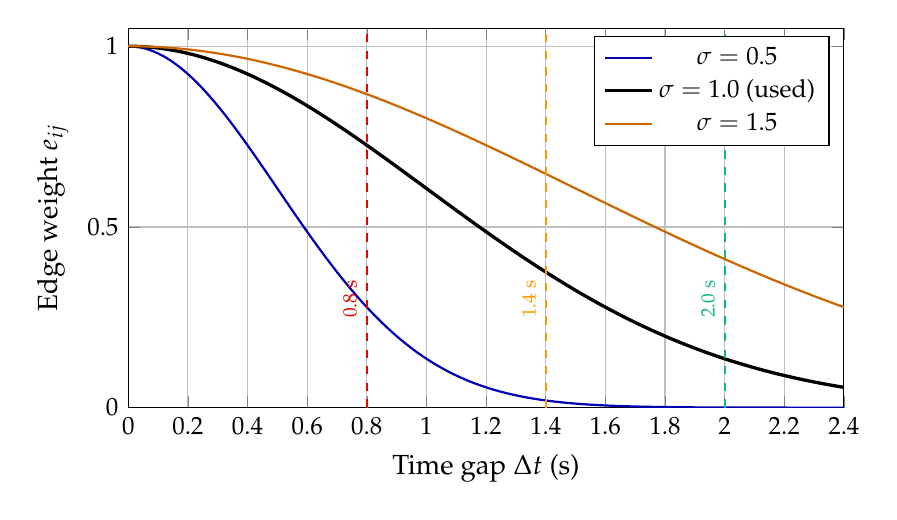
\begin{tikzpicture}
\begin{axis}[
  width=0.88\linewidth, height=6.4cm,
  xlabel={Time gap $\Delta t$ (s)}, ylabel={Edge weight $e_{ij}$},
  xmin=0, xmax=2.4, ymin=0, ymax=1.05,
  domain=0:2.4, samples=120, grid=both,
  legend style={at={(0.98,0.98)},anchor=north east,font=\small},
  tick label style={font=\small}
]
\addplot[thick,blue!70!black] {exp(-x^2/(2*0.5^2))};
\addplot[very thick,black] {exp(-x^2/(2*1.0^2))};
\addplot[thick,orange!80!black] {exp(-x^2/(2*1.5^2))};
\legend{$\sigma=0.5$,$\sigma=1.0$ (used),$\sigma=1.5$}
\draw[dashed,f1red,thick] (axis cs:0.8,0) -- (axis cs:0.8,1.05);
\draw[dashed,f1orange,thick] (axis cs:1.4,0) -- (axis cs:1.4,1.05);
\draw[dashed,f1green,thick] (axis cs:2.0,0) -- (axis cs:2.0,1.05);
\node[font=\scriptsize,f1red,rotate=90,anchor=south] at (axis cs:0.8,0.3) {0.8 s};
\node[font=\scriptsize,f1orange,rotate=90,anchor=south] at (axis cs:1.4,0.3) {1.4 s};
\node[font=\scriptsize,f1green,rotate=90,anchor=south] at (axis cs:2.0,0.3) {2.0 s};
\end{axis}
\end{tikzpicture}
\caption{Gaussian RBF edge weight for three kernel widths. The dashed lines mark the tier limits and the edge limit at 2~s.}
\label{fig:rbf}
\end{figure}

\subsection{Kernel Width Sensitivity}
The width $\sigma$ controls how fast the influence falls with the gap.
Table~\ref{tab:sigma} shows the weights for selected gaps (computed from the
formula). With $\sigma = 0.5$~s the weight at 1.5~s is almost zero, and the
2~s limit would be meaningless. With $\sigma=1.5$~s the weight at 2~s is still
0.41, so the cut-off at 2~s would create a visible step. The value
$\sigma=1.0$~s gives a weight of 0.135 at the limit, which is a gentle cut-off.
A study of $\sigma$ is planned in the experiments of Section~\ref{sec:future}.

\begin{table}[H]
\centering
\caption{Edge weight $e_{ij}$ for selected gaps and kernel widths.}
\label{tab:sigma}
\small
\begin{tabular}{@{}lcccc@{}}
\toprule
\textbf{Kernel width} & $\dt=0.5$ s & $\dt=1.0$ s & $\dt=1.5$ s & $\dt=2.0$ s \\
\midrule
$\sigma = 0.5$ s & 0.6065 & 0.1353 & 0.0111 & 0.0003 \\
$\sigma = 1.0$ s (used) & 0.8825 & 0.6065 & 0.3247 & 0.1353 \\
$\sigma = 1.5$ s & 0.9460 & 0.8007 & 0.6065 & 0.4111 \\
\bottomrule
\end{tabular}
\end{table}

\subsection{Disturbance Tiers}
For display and analysis, edges are grouped in three tiers. The thresholds on
$e_{ij}$ follow from the thresholds on the gap, with $\sigma=1$:
$e(0.8)=0.726$, $e(1.4)=0.375$, $e(2.0)=0.135$. The inverse of the kernel,
$\dt = \sqrt{-2\sigma^2\ln e}$, recovers the gap from a stored weight, and the
visualiser uses this to label the arrows.

\begin{table}[H]
\centering
\caption{Disturbance tiers used for graph visualisation.}
\label{tab:tiers}
\small
\begin{tabularx}{\linewidth}{@{}l l c c X@{}}
\toprule
\textbf{Tier} & \textbf{Colour} & \textbf{Gap $\Delta t$} & \textbf{Weight $e_{ij}$} & \textbf{Meaning} \\
\midrule
Severe dirty air & \cellcolor{f1red!35}Red    & $<0.8$ s         & $\ge 0.726$        & Strong wake, DRS-train range \\
Moderate wake    & \cellcolor{f1orange!35}Orange & $0.8$--$1.4$ s & $0.375$--$0.726$   & Noticeable disturbance \\
Light wake       & \cellcolor{f1green!35}Green & $1.4$--$2.0$ s  & $0.135$--$0.375$   & Minor disturbance \\
Clean air        & ---    & $>2.0$ s         & $0$ (no edge)      & No disturbance \\
\bottomrule
\end{tabularx}
\end{table}
\noindent\emph{Note.} The project documents attach indicative downforce-loss
percentages to the tiers. These are design assumptions. They have not been
measured or validated in this work, and this report does not rely on them.

\subsection{Node Features}
Each node (car) has four normalised features:
\begin{equation}
\mathbf{x}_i = \Bigl[\tfrac{\text{Speed}}{320},\; \tfrac{\text{Throttle}}{100},\;
\tfrac{\text{TyreLife}}{55},\; \tfrac{\text{MiniSector}}{20}\Bigr].
\end{equation}
Normalisation keeps all inputs in a similar range, which makes training stable.
Note that the sector index appears as a single scaled number, so the model
must learn the (non-linear) effect of the track position itself.

\subsection{Construction Algorithm}
\begin{algorithm}[H]
\caption{Build the graph snapshot at time $t$}
\label{alg:graph}
\begin{algorithmic}[1]
\Require Rows at time $t$; threshold $g_{\max}=2.0$; width $\sigma=1.0$; index map $\pi$ (driver $\to$ node)
\Ensure Snapshot $(\mathbf{X}_t,\ \mathcal{E}_t,\ \mathbf{e}_t)$
\State $\mathbf{X}_t \gets \mathbf{0} \in \mathbb{R}^{N\times 4}$; \ $\mathcal{E}_t \gets \emptyset$
\For{each row $r$ at time $t$}
  \State $i \gets \pi(r.\text{Driver})$
  \State $\mathbf{X}_t[i] \gets [\,r.\text{Speed}/320,\ r.\text{Throttle}/100,\ r.\text{TyreLife}/55,\ r.\text{MiniSector}/20\,]$
  \State $j \gets \pi(r.\text{DriverAhead})$;\ \ $g \gets r.\text{DeltaT}$
  \If{$j$ exists \textbf{and} $0 < g \le g_{\max}$}
    \State add edge $(j \to i)$ with weight $\exp(-g^2/2\sigma^2)$
  \EndIf
\EndFor
\end{algorithmic}
\end{algorithm}

\subsection{Structural Property: The Graph is a Set of Chains}
Because each car has an edge only to the car \emph{directly} ahead, every node
has at most one incoming edge and at most one outgoing edge. The graph at any
time step is therefore a collection of directed paths (``chains'') plus
isolated cars. This has two practical consequences. The adjacency matrix has
at most one non-zero entry in each row and each column (visible in
Figure~\ref{fig:graph}). And a model that uses a single message-passing layer
sees only the immediate leader of each car. The cumulative effect of a long
train (the leader's leader, and so on) can reach a car only through multiple
hops or through the temporal dimension.

\subsection{Graph Statistics}
\begin{table}[H]
\centering
\caption{Output of the graph construction stage.}
\label{tab:graphstats}
\small
\begin{tabular}{@{}lr@{}}
\toprule
\textbf{Quantity} & \textbf{Value} \\
\midrule
Aligned telemetry rows & 416{,}879 \\
Drivers (nodes per graph) & 19 \\
Graph snapshots (4 Hz) & 21{,}941 \\
Total directed edges & 137{,}355 \\
Average active edges per snapshot & 6.26 \\
Maximum possible edges per snapshot (chain of 19 cars) & 18 \\
Mini-sector target segments & 19{,}768 \\
\bottomrule
\end{tabular}
\end{table}
On average, about one third of the possible ``follower slots'' carry an edge
($6.26 / 18 \approx 0.35$). The rest of the time, cars run more than 2~s behind
the car ahead.

\subsection{Worked Example}
Consider a follower 0.60~s behind its leader. The weight is
$e = \exp(-0.60^2 / 2) = \exp(-0.18) \approx 0.835$, which is above 0.726, so
the edge is red. For a gap of 1.30~s, $e = \exp(-0.845) \approx 0.430$. This is
between 0.375 and 0.726, so the edge is orange. The latter value is the one
that appears for the pair \texttt{31 OCO} $\to$ \texttt{3 RIC} in
Table~\ref{tab:edges}.

% =====================================================================
\section{Model: CoreSTGNN}
\label{sec:model}
% =====================================================================

\subsection{Architecture Overview}
\begin{figure}[H]
\centering
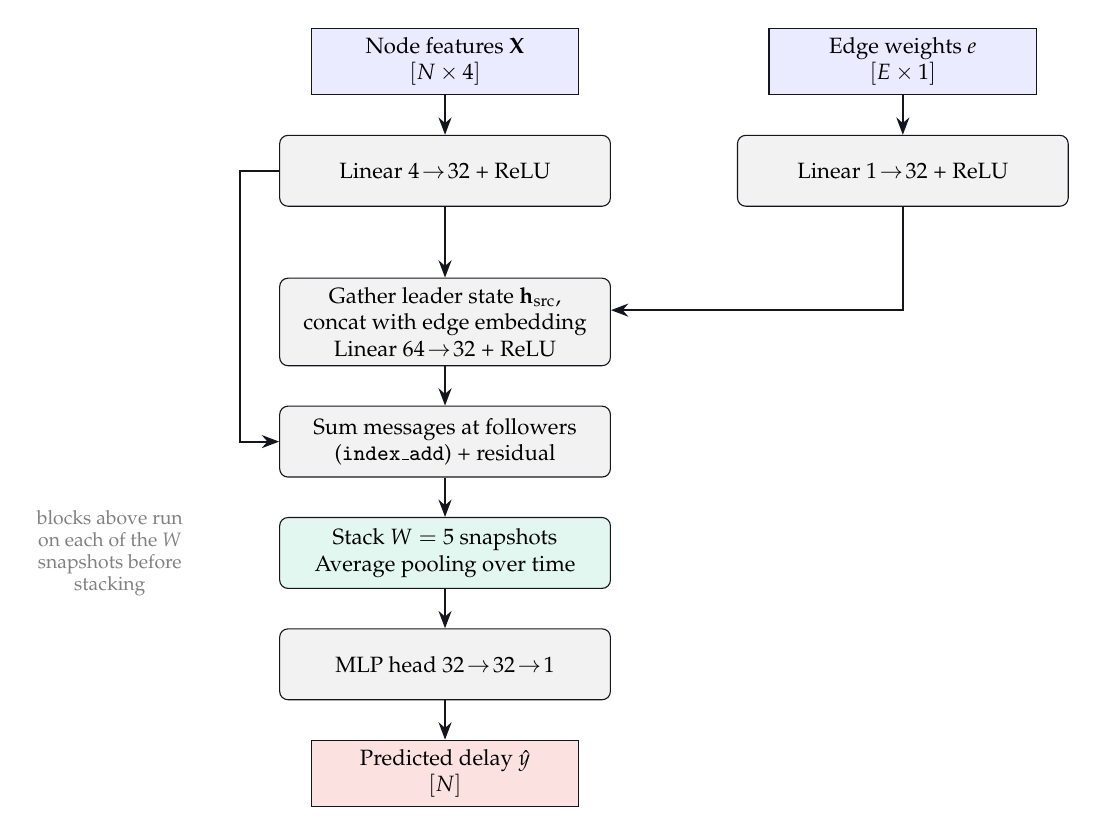
\begin{tikzpicture}[
  node distance=0.5cm and 0.9cm,
  blk/.style={rectangle,rounded corners=3pt,draw=carbon,fill=gray!10,minimum height=0.9cm,
              minimum width=4.2cm,align=center,font=\footnotesize},
  io/.style={rectangle,draw=carbon,fill=blue!8,minimum height=0.8cm,minimum width=3.4cm,
             align=center,font=\footnotesize},
  arr/.style={-{Stealth[length=2.2mm]},thick,carbon}
]
\node[io] (x) {Node features $\mathbf{X}$\\ $[N \times 4]$};
\node[blk,below=of x] (p) {Linear $4\!\to\!32$ + ReLU};
\node[io,right=2.4cm of x] (e) {Edge weights $e$\\ $[E \times 1]$};
\node[blk,below=of e] (ee) {Linear $1\!\to\!32$ + ReLU};
\node[blk,below=0.9cm of p] (m) {Gather leader state $\mathbf{h}_{\text{src}}$,\\ concat with edge embedding\\ Linear $64\!\to\!32$ + ReLU};
\node[blk,below=of m] (a) {Sum messages at followers\\ (\texttt{index\_add}) + residual};
\node[blk,below=of a,fill=f1green!12] (t) {Stack $W=5$ snapshots\\ Average pooling over time};
\node[blk,below=of t] (h) {MLP head $32\!\to\!32\!\to\!1$};
\node[io,below=of h,fill=f1red!12] (y) {Predicted delay $\hat{y}$\\ $[N]$};
\draw[arr] (x)--(p);
\draw[arr] (e)--(ee);
\draw[arr] (p)--(m);
\draw[arr] (ee.south) |- ($(m.east)+(0,0.15)$);
\draw[arr] (m)--(a);
\draw[arr] (p.west) -- ++(-0.5,0) |- (a.west);
\draw[arr] (a)--(t);
\draw[arr] (t)--(h);
\draw[arr] (h)--(y);
\node[font=\scriptsize,gray,align=center,left=0.1cm of t,xshift=-1.0cm] {blocks above run\\ on each of the $W$\\ snapshots before\\ stacking};
\end{tikzpicture}
\caption{Architecture of \texttt{CoreSTGNN}. The spatial part (projection and message passing) runs on every snapshot of the window. The results are pooled over time and mapped to one delay value per car.}
\label{fig:model}
\end{figure}

\subsection{Spatial Message Passing}
For each snapshot, node states are first projected:
\begin{equation}
\mathbf{h}_i^{(0)} = \operatorname{ReLU}(W_p\,\mathbf{x}_i + b_p), \qquad \mathbf{h}_i \in \mathbb{R}^{32}.
\end{equation}
For every edge $(j \rightarrow i)$, the edge weight is embedded and combined with
the leader state to form a message. The messages are summed at the follower,
and the sum is added to the follower's own state (a residual connection):
\begin{align}
\mathbf{m}_{ji} &= \operatorname{ReLU}\!\bigl(W_m\,[\,\mathbf{h}_j \,\|\, \operatorname{ReLU}(W_e\, e_{ji} + b_e)\,] + b_m\bigr),\\
\mathbf{h}_i' &= \mathbf{h}_i + \sum_{j \in \mathcal{N}(i)} \mathbf{m}_{ji}.
\end{align}
Here $\mathcal{N}(i)$ is the set of leaders of car $i$. In this graph it has at
most one element (Section~\ref{sec:graph}). The sum is still written in general
form, because the 100\% version may allow more than one leader.

\subsection{Temporal Pooling}
The states of the $W = 5$ snapshots of a window are stacked and averaged over time:
\begin{equation}
\bar{\mathbf{h}}_i = \frac{1}{W}\sum_{w=1}^{W} \mathbf{h}_i'^{\,(w)}.
\end{equation}
The mean treats all snapshots as equally important and ignores their order.
It cannot represent a trend (for example, a gap that closes quickly). A
temporal convolution is planned to fix this.

\subsection{Regression Head}
A two-layer perceptron ($32 \rightarrow 32 \rightarrow 1$ with ReLU) maps
$\bar{\mathbf{h}}_i$ to the predicted delay $\hat{y}_i$.

\subsection{Parameter Count}
\begin{table}[H]
\centering
\caption{Layers and trainable parameters of \texttt{CoreSTGNN}.}
\label{tab:params}
\small
\begin{tabular}{@{}lllr@{}}
\toprule
\textbf{Layer} & \textbf{Mapping} & \textbf{Formula} & \textbf{Parameters} \\
\midrule
\texttt{proj} & $4 \to 32$ & $4\cdot32+32$ & 160 \\
\texttt{edge\_proj} & $1 \to 32$ & $1\cdot32+32$ & 64 \\
\texttt{msg\_layer} & $64 \to 32$ & $64\cdot32+32$ & 2{,}080 \\
\texttt{head[0]} & $32 \to 32$ & $32\cdot32+32$ & 1{,}056 \\
\texttt{head[2]} & $32 \to 1$ & $32\cdot1+1$ & 33 \\
\midrule
\multicolumn{3}{@{}l}{\textbf{Total}} & \textbf{3{,}393} \\
\bottomrule
\end{tabular}
\end{table}
The temporal pooling layer has no parameters.

\subsection{Computational Cost}
For a sample with $W$ snapshots, $N$ nodes and $E$ edges per snapshot, the
cost of the forward pass is $\mathcal{O}\bigl(W\,(N\,F\,D + E\,D^2)\bigr)$.
With $N=19$, $E\approx 6$, $D=32$ and $W=5$, this is a few hundred thousand
operations per sample, which explains why one epoch over 4{,}112 samples
finishes in seconds on a CPU. The gap computation of Algorithm~\ref{alg:gap}
is more expensive in the current implementation, because it looks up the rows
of the leader and the follower with a boolean filter at every step. Its cost
is quadratic in $N$ per time step, which is acceptable for 19 cars and cached
after the first run.

\subsection{Limits of the Core Design}
\begin{itemize}[leftmargin=*]
  \item \textbf{One hop.} One layer sees only the direct leader. A car that is
        third in a train cannot see the first car.
  \item \textbf{No learned attention.} All edges contribute through their
        weight embedding only; the model cannot decide that one leader matters
        more than another.
  \item \textbf{No order in time.} Average pooling ignores the order of the
        snapshots.
  \item \textbf{Weak inputs.} Four features, a constant compound and no
        pit-lap information.
\end{itemize}
These limits are the main reason for the 100\% architecture of
Section~\ref{sec:future}.

% =====================================================================
\section{Experimental Setup}
\label{sec:setup}
% =====================================================================

\subsection{Training Samples}
A training sample is a window of $W=5$ consecutive snapshots paired with the
target of the snapshot with index $i+W+K$, where $i$ is the first snapshot of
the window and $K=5$. The last snapshot of the window has index $i+W-1$, so
the target lies $K+1 = 6$ snapshots (1.5~s) after the last input. Windows
start every 4 snapshots (1~s). Figure~\ref{fig:window} shows the layout.

\begin{figure}[H]
\centering
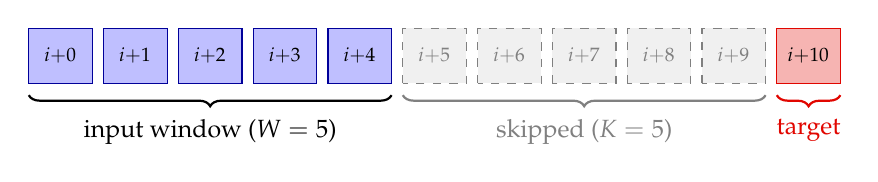
\begin{tikzpicture}[x=0.95cm,y=1cm]
\foreach \k in {0,...,4}{
  \draw[fill=blue!25,draw=blue!60!black] (\k,0) rectangle ++(0.85,0.7);
  \node[font=\scriptsize] at (\k+0.42,0.35) {$i{+}\k$};
}
\foreach \k in {5,...,9}{
  \draw[fill=gray!12,draw=gray,dashed] (\k,0) rectangle ++(0.85,0.7);
  \node[font=\scriptsize,gray] at (\k+0.42,0.35) {$i{+}\k$};
}
\draw[fill=f1red!30,draw=f1red] (10,0) rectangle ++(0.85,0.7);
\node[font=\scriptsize] at (10.42,0.35) {$i{+}10$};
\draw[decorate,decoration={brace,amplitude=4pt,mirror},thick] (0,-0.15) -- (4.85,-0.15)
  node[midway,below=5pt,font=\small] {input window ($W=5$)};
\draw[decorate,decoration={brace,amplitude=4pt,mirror},thick,gray] (5,-0.15) -- (9.85,-0.15)
  node[midway,below=5pt,font=\small,gray] {skipped ($K=5$)};
\draw[decorate,decoration={brace,amplitude=4pt,mirror},thick,f1red] (10,-0.15) -- (10.85,-0.15)
  node[midway,below=5pt,font=\small,f1red] {target};
\end{tikzpicture}
\caption{Layout of one training sample. Each box is one 0.25~s snapshot.}
\label{fig:window}
\end{figure}

The construction yields 5{,}483 samples; every window had at least two
labelled cars. Algorithm~\ref{alg:dataset} summarises the process.

\begin{algorithm}[H]
\caption{Build the window dataset}
\label{alg:dataset}
\begin{algorithmic}[1]
\Require Snapshots $\mathcal{S}_0,\dots,\mathcal{S}_{T-1}$; target table; $W=5$, $K=5$, stride 4
\Ensure List of samples (window, target vector $\mathbf{y}$, mask $\mathbf{m}$)
\For{$i = 0,\ 4,\ 8,\ \dots,\ T - W - K - 1$}
  \State window $\gets \mathcal{S}_i,\dots,\mathcal{S}_{i+W-1}$;\quad target snapshot $\gets \mathcal{S}_{i+W+K}$
  \For{each driver $d$ with node index $n$}
    \State $s \gets$ mini-sector of $d$ in the target snapshot
    \State look up the label of $(d, s)$ in the target table
    \If{a label exists} \ $y_n \gets$ label;\ $m_n \gets 1$ \Else \ $m_n \gets 0$ \EndIf
  \EndFor
  \If{$\sum_n m_n \ge 2$} \ store the sample \EndIf
\EndFor
\end{algorithmic}
\end{algorithm}

\subsection{Data Split}
The samples are split chronologically: the first 75\% (4{,}112 windows,
roughly laps 1--43) train the model, and the last 25\% (1{,}371 windows,
roughly laps 44--58) test it. The lap ranges are approximate, because the
split is by sample index and not by lap boundary.

\subsection{Hyper-parameters}
\begin{table}[H]
\centering
\caption{Hyper-parameters of the core experiment.}
\label{tab:hparams}
\small
\begin{tabular}{@{}ll@{}}
\toprule
\textbf{Parameter} & \textbf{Value} \\
\midrule
Input dimension $F$ & 4 \\
Hidden dimension $D$ & 32 \\
Window length $W$ / offset $K$ & 5 / 5 snapshots \\
Window stride & 4 snapshots (1 s) \\
Edge threshold / kernel width $\sigma$ & 2.0 s / 1.0 s \\
Optimiser & Adam, learning rate $3\times10^{-3}$, weight decay $10^{-4}$ \\
Loss & Masked L1 \\
Batch size & 1 window per optimiser step \\
Epochs & 10 (full run); 3 (quick run in Fig.~\ref{fig:terminal}) \\
Sampling rate & 4 Hz \\
Random seed & Not fixed in the current code \\
\bottomrule
\end{tabular}
\end{table}

\subsection{Loss and Metrics}
Not every car has a target in every window, so a mask $m_i \in \{0,1\}$ is
used, and the loss is the masked mean absolute error:
\begin{equation}
\mathcal{L} = \frac{\sum_i m_i\,|\hat{y}_i - y_i|}{\max\bigl(\sum_i m_i,\,1\bigr)}.
\end{equation}
Test quality is reported with the mean absolute error and the coefficient of
determination, both computed over all labelled (window, car) pairs of the test set:
\begin{equation}
\text{MAE} = \frac{1}{n}\sum_{k}|\hat{y}_k - y_k|, \qquad
R^2 = 1 - \frac{\sum_k (y_k-\hat{y}_k)^2}{\sum_k (y_k-\bar{y})^2}.
\end{equation}
$R^2=0$ corresponds to always predicting the mean of the test labels, and
$R^2=1$ to a perfect prediction. A value of $0.29$ therefore means that the
model explains about 29\% of the variance of the labels beyond a constant
prediction.

\subsection{Reproducibility and Commands}
\begin{lstlisting}[language=bash]
# graph building and visualisation only (about 23 s with cache)
uv run python hammertime_50/demo_core.py --mode graph --snapshot-idx 3000

# full pipeline: graph + training + evaluation + analytics
uv run python hammertime_50/demo_core.py --mode full --epochs 10

# use synthetic telemetry instead of the real race
uv run python hammertime_50/demo_core.py --synthetic --mode full
\end{lstlisting}
The Parquet cache makes the data stage deterministic after the first
download. The training stage is \emph{not} yet fully deterministic, because
the random seed is not fixed (this is recorded in the plan).

\subsection{Runtime}
\begin{table}[H]
\centering
\caption{Stage timing taken from the execution log (3-epoch run, cached data).}
\label{tab:runtime}
\small
\begin{tabular}{@{}lr@{}}
\toprule
\textbf{Stage} & \textbf{Time} \\
\midrule
Load cached Parquet $\to$ clean-air targets ready & about 1.5 s after load \\
Build 21{,}941 graph snapshots & about 25 s \\
Dataset build, 3 epochs, evaluation, analytics & about 80 s (remainder) \\
\textbf{Total} & \textbf{113.24 s} \\
\bottomrule
\end{tabular}
\end{table}

% =====================================================================
\section{Results}
\label{sec:results}
% =====================================================================

\subsection{Execution Log}
Figure~\ref{fig:terminal} shows a complete run of the pipeline with 3 epochs.
All five stages finish without error. The only warning is a harmless
font-weight message from the plotting library.

\begin{figure}[H]
\centering
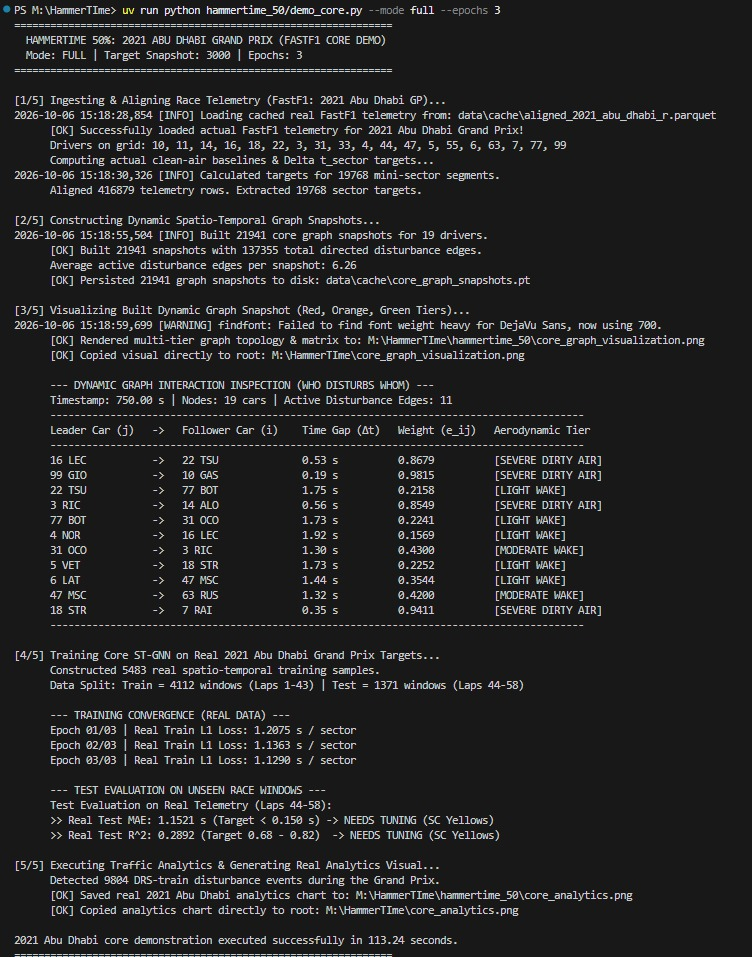
\includegraphics[width=0.82\linewidth,height=0.62\textheight,keepaspectratio]{terminal_run.jpg}
\caption{Terminal output of \texttt{demo\_core.py -{}-mode full -{}-epochs 3}.}
\label{fig:terminal}
\end{figure}

\subsection{Dynamic Graph Snapshot}
Snapshot 3000 (time $t = 750$~s, about lap 8) has 11 active edges: 4 red,
2 orange and 5 green. Figure~\ref{fig:graph} shows the circular topology on
the left, with arrows from leader to follower and team colours on the node
rings, and the weighted adjacency matrix $A[\text{leader},\text{follower}]$
on the right.

\begin{figure}[H]
\centering
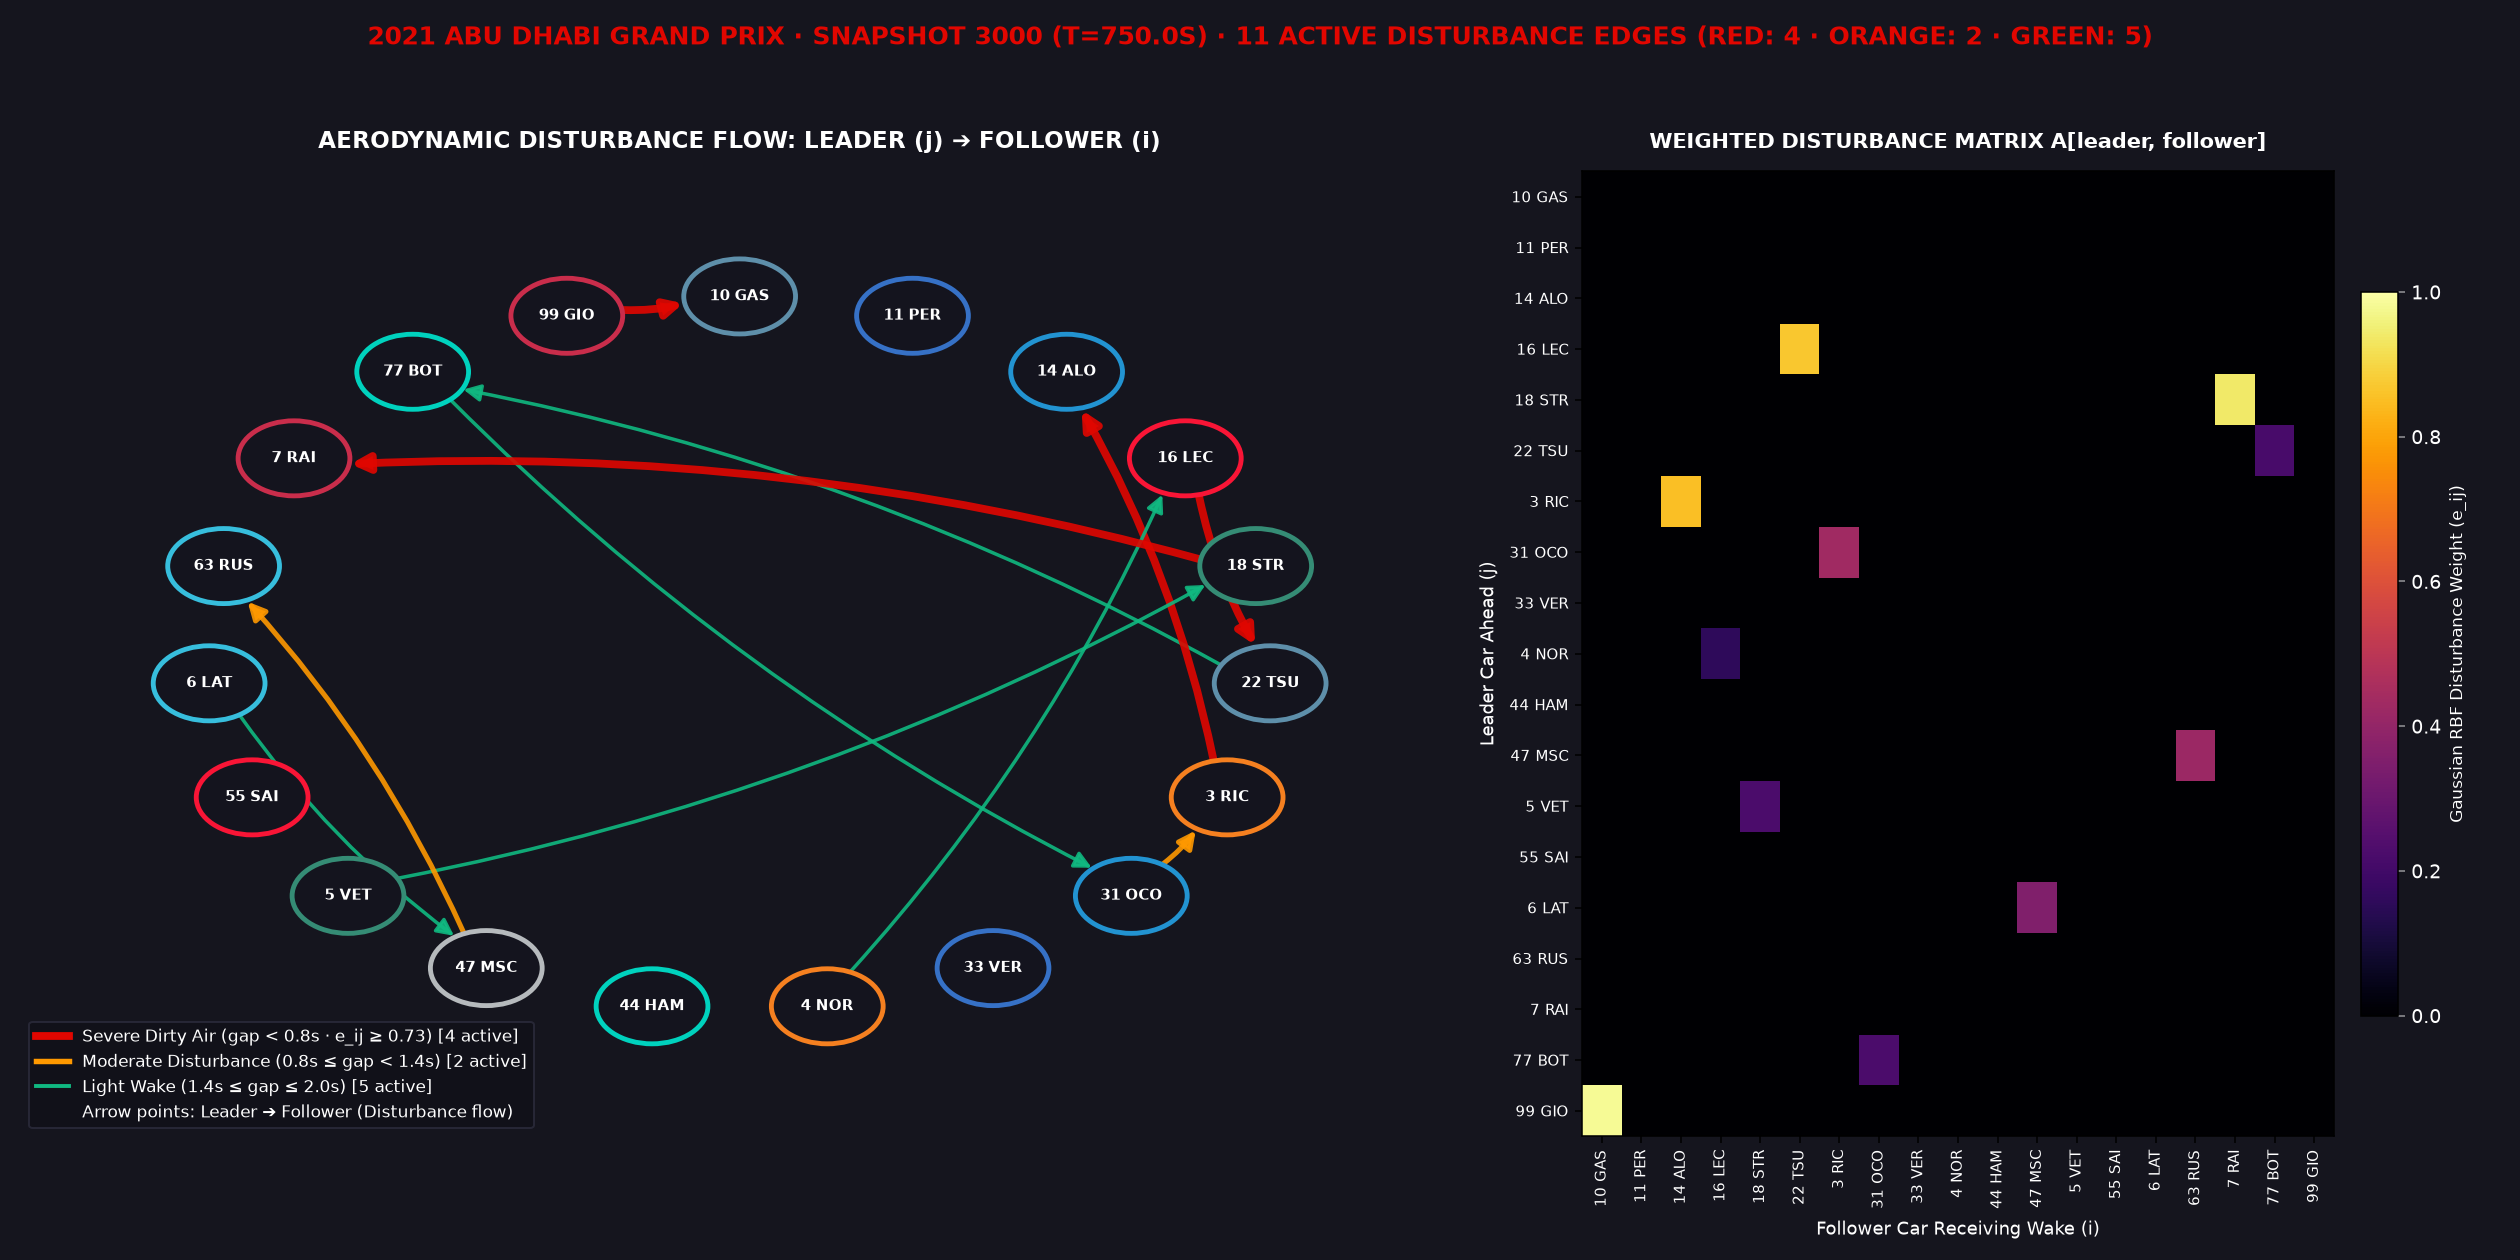
\includegraphics[width=\linewidth]{graph_snapshot.png}
\caption{Dynamic disturbance graph at snapshot 3000 ($t = 750$~s).}
\label{fig:graph}
\end{figure}

\begin{table}[H]
\centering
\caption{Active edges at snapshot 3000. Gaps are rounded to two decimals in the log.}
\label{tab:edges}
\small
\begin{tabular}{@{}llccl@{}}
\toprule
\textbf{Leader $j$} & \textbf{Follower $i$} & \textbf{Gap (s)} & \textbf{$e_{ij}$} & \textbf{Tier} \\
\midrule
99 GIO & 10 GAS & 0.19 & 0.9815 & \cellcolor{f1red!35}Severe \\
18 STR & 7 RAI  & 0.35 & 0.9411 & \cellcolor{f1red!35}Severe \\
16 LEC & 22 TSU & 0.53 & 0.8679 & \cellcolor{f1red!35}Severe \\
3 RIC  & 14 ALO & 0.56 & 0.8549 & \cellcolor{f1red!35}Severe \\
31 OCO & 3 RIC  & 1.30 & 0.4300 & \cellcolor{f1orange!35}Moderate \\
47 MSC & 63 RUS & 1.32 & 0.4200 & \cellcolor{f1orange!35}Moderate \\
6 LAT  & 47 MSC & 1.44 & 0.3544 & \cellcolor{f1green!35}Light \\
77 BOT & 31 OCO & 1.73 & 0.2241 & \cellcolor{f1green!35}Light \\
5 VET  & 18 STR & 1.73 & 0.2252 & \cellcolor{f1green!35}Light \\
22 TSU & 77 BOT & 1.75 & 0.2158 & \cellcolor{f1green!35}Light \\
4 NOR  & 16 LEC & 1.92 & 0.1569 & \cellcolor{f1green!35}Light \\
\bottomrule
\end{tabular}
\end{table}

\subsubsection{Reading the Snapshot}
The 11 edges link cars into chains. Following the arrows gives
\begin{itemize}[leftmargin=*]
  \item a chain of seven cars:
        \texttt{4 NOR} $\to$ \texttt{16 LEC} $\to$ \texttt{22 TSU} $\to$
        \texttt{77 BOT} $\to$ \texttt{31 OCO} $\to$ \texttt{3 RIC} $\to$
        \texttt{14 ALO} (gaps 1.92, 0.53, 1.75, 1.73, 1.30, 0.56~s);
  \item two chains of three cars:
        \texttt{5 VET} $\to$ \texttt{18 STR} $\to$ \texttt{7 RAI}, and
        \texttt{6 LAT} $\to$ \texttt{47 MSC} $\to$ \texttt{63 RUS};
  \item one pair, \texttt{99 GIO} $\to$ \texttt{10 GAS};
  \item four isolated cars: \texttt{33 VER}, \texttt{44 HAM}, \texttt{11 PER}
        and \texttt{55 SAI}. They have no car within 2~s ahead.
\end{itemize}
These are 15 connected cars and 4 isolated ones, which agrees with 11 edges
(a chain of $n$ cars has $n-1$ edges: $6+2+2+1=11$). Each leader and each
follower appears exactly once in Table~\ref{tab:edges}, which agrees with the
at-most-one-in, at-most-one-out property. The tier of every edge agrees with
the thresholds of Table~\ref{tab:tiers}.

None of the chains contains three consecutive red edges, so a DRS train in the
sense of the detector (a chain of at least three cars with every gap $\le 0.8$~s)
is not present at this moment. The nearest case is the pair
\texttt{16 LEC}~$\to$~\texttt{22 TSU} (red), followed by a light edge to
\texttt{77 BOT}.

\subsection{DRS-Train Detection}
The detector reports 9{,}804 events over the race. An event is counted at each
time step at which a chain of at least three cars with gaps of at most 0.8~s
exists. Consecutive steps of the same train are therefore counted separately,
and the figure is an upper bound on the number of distinct trains, not a
count of trains. A grouping step over consecutive time steps is needed to
report distinct trains and their duration (planned in the 100\% version,
visual V4).

\subsection{Training Convergence}
\begin{table}[H]
\centering
\caption{Training loss (masked L1, seconds per sector).}
\label{tab:loss}
\small
\begin{tabular}{@{}lccccc@{}}
\toprule
\textbf{Epoch} & 1 & 2 & 4 & 7 & 10 \\
\midrule
10-epoch run & 1.2110 & 1.1405 & 1.1283 & 1.1110 & 1.1052 \\
\bottomrule
\end{tabular}

\vspace{1mm}
\begin{tabular}{@{}lccc@{}}
\toprule
\textbf{Epoch} & 1 & 2 & 3 \\
\midrule
3-epoch run (Fig.~\ref{fig:terminal}) & 1.2075 & 1.1363 & 1.1290 \\
\bottomrule
\end{tabular}
\end{table}
The loss decreases monotonically in both runs, which shows that the
optimisation works. Most of the improvement happens in the first two epochs;
after that the curve is almost flat at about 1.1~s.

\begin{figure}[H]
\centering
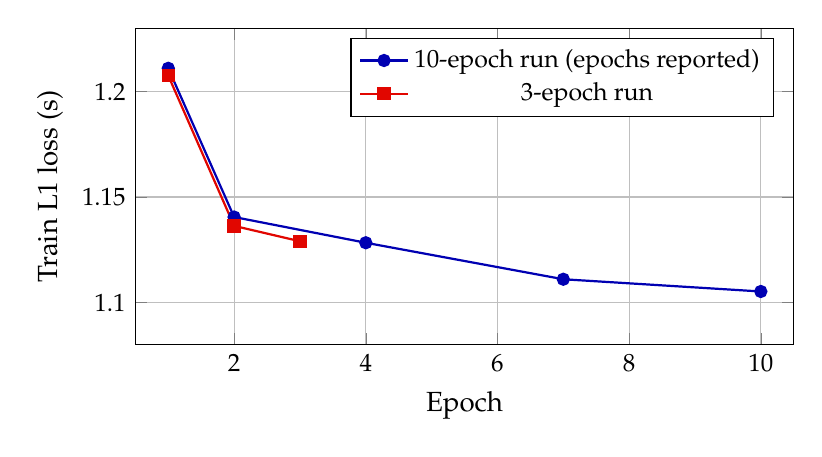
\begin{tikzpicture}
\begin{axis}[
  width=0.82\linewidth, height=5.6cm,
  xlabel={Epoch}, ylabel={Train L1 loss (s)},
  xmin=0.5, xmax=10.5, ymin=1.08, ymax=1.23,
  grid=both, legend style={font=\small,at={(0.97,0.97)},anchor=north east},
  tick label style={font=\small}
]
\addplot[thick,mark=*,blue!70!black] coordinates {(1,1.2110)(2,1.1405)(4,1.1283)(7,1.1110)(10,1.1052)};
\addplot[thick,mark=square*,f1red] coordinates {(1,1.2075)(2,1.1363)(3,1.1290)};
\legend{10-epoch run (epochs reported),3-epoch run}
\end{axis}
\end{tikzpicture}
\caption{Training loss of the two runs (only the epochs listed in the reports are plotted).}
\label{fig:loss}
\end{figure}

\subsection{Test Performance}
\begin{table}[H]
\centering
\caption{Performance on the held-out closing windows (laps 44--58).}
\label{tab:metrics}
\small
\begin{tabular}{@{}lccc@{}}
\toprule
\textbf{Metric} & \textbf{Target} & \textbf{10 epochs} & \textbf{3 epochs} \\
\midrule
Test MAE (s) & $< 0.150$ & 1.1407 & 1.1521 \\
Test $R^2$ & $0.68$--$0.82$ & 0.2943 & 0.2892 \\
\bottomrule
\end{tabular}
\end{table}

\subsection{Traffic Analytics}
\begin{figure}[H]
\centering
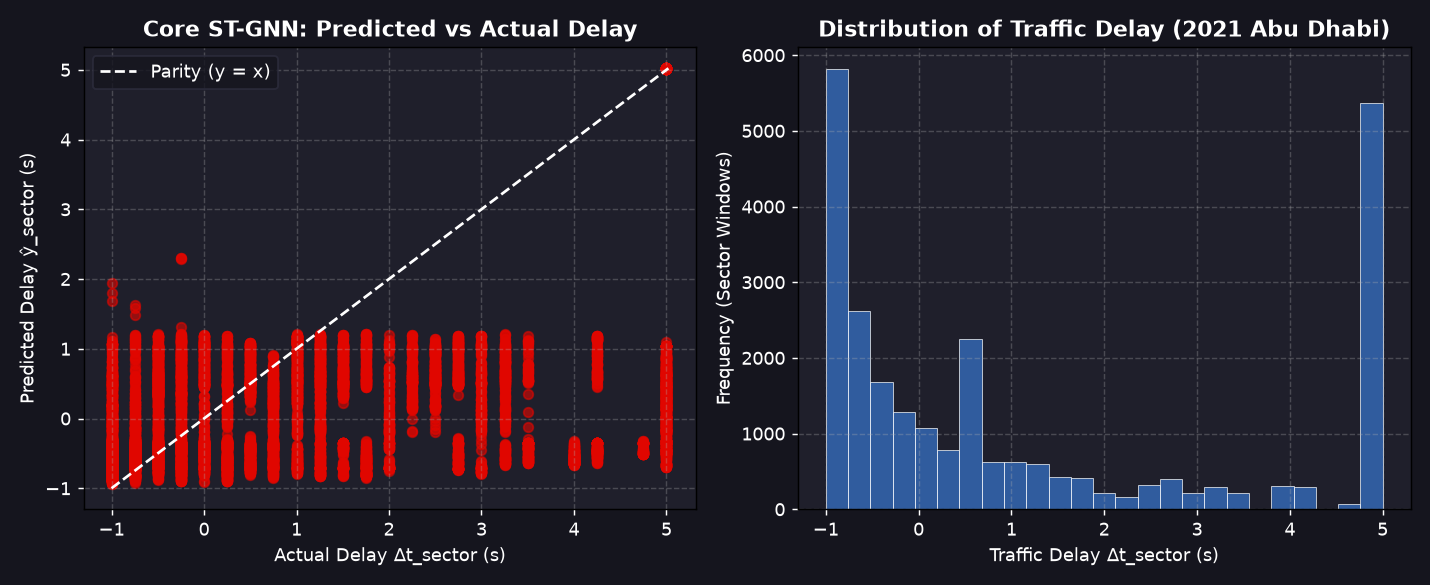
\includegraphics[width=\linewidth]{analytics.png}
\caption{Left: predicted versus actual delay on the test windows (the dashed line is parity). Right: distribution of the actual delay in the test windows.}
\label{fig:analytics}
\end{figure}

Both panels of Figure~\ref{fig:analytics} are computed from the test windows
only, because the plotting function receives the test labels and predictions.
(The project README describes the histogram as covering the whole race. This
should be corrected in the next iteration.)

\subsubsection{Left Panel: Parity Plot}
Points on the dashed line would be perfect predictions. The cloud is instead a
set of vertical stripes. All predictions lie between about $-1$ and $1.2$~s
whatever the actual value, and the stripe at $+5$~s (the clip limit) is
predicted at the same level as the stripe at $-1$~s. The model has learned
roughly a constant with a small spread and does not follow the large
delays. The vertical stripes appear because actual values are multiples of
0.25~s (quantisation, Section~\ref{sec:data}).

\subsubsection{Right Panel: Label Distribution}
The distribution is bimodal. About 5{,}800 samples sit at the lowest bin near
$-1$~s (the lower clip limit), and about 5{,}400 at the upper limit near
$+5$~s. A third, small peak appears near $0.5$~s. Between these, the
frequency falls slowly. So a large part of the labels lie \emph{on a clip
limit}. For such samples, the true unclipped value is unknown, and the
delay they encode is either very small or very large, not typical.

\subsection{Interpretation of the Train--Test Gap}
The final training loss ($1.105$~s) and the test MAE ($1.141$~s) are close. A
close pair of numbers normally indicates under-fitting (the model is too
simple, or the input does not contain the information) and not over-fitting.
This reading must be used with care for two reasons. The two numbers are
computed differently (a mean of per-window means, and a pooled mean), and the
label look-up in this version gives the same label for the same (driver,
sector) in the training and in the test windows (Section~\ref{sec:analysis}).

% =====================================================================
\section{Analysis, Limitations and Threats to Validity}
\label{sec:analysis}
% =====================================================================
This section lists the causes that may explain the gap between the results and
the targets. They are ordered by the evidence available. Two are confirmed by
reading the code; the others are hypotheses that the second half will test.

\subsection{Findings}
\begin{enumerate}[leftmargin=*]
  \item \textbf{Label look-up is not lap-aware (confirmed by code
        inspection).} The training-set builder creates a dictionary keyed by
        (driver, mini-sector) and fills it by looping over all target rows.
        The rows are sorted by driver, then lap. Each assignment overwrites
        the previous one, so the stored label of a (driver, sector) pair is
        the value from that driver's \emph{last lap}. Every sample, in the
        training and in the test set, then receives that same value for the
        same (driver, sector), whatever the lap of the target snapshot is
        (Appendix~\ref{app:code}). The consequences are:
        \begin{itemize}
          \item the labels do not describe the traffic at the time of the
                sample, so the model cannot learn the real link between
                traffic and delay;
          \item the same label appears in both partitions, so the chronological
                split does not prevent label overlap between train and test;
          \item the last lap of the race follows the Safety Car, and its
                sector times can be very large; this may explain part of the
                mass at $+5$~s in Figure~\ref{fig:analytics}.
        \end{itemize}
        The fix is to key the dictionary by (driver, lap, mini-sector), and
        to read the lap of the target snapshot.
  \item \textbf{Sector index from a float product (confirmed by code
        inspection, minor).} The sector of the target snapshot is recovered
        as \texttt{int(x * 20.0)} from a 32-bit float that stores $s/20$.
        Truncation can map a sector $s$ to $s-1$ for some values of $s$. The
        fix is to store the integer sector separately, or to round.
  \item \textbf{Safety Car period (diagnosed, not yet quantified).} On
        lap~53 the Safety Car was deployed after the crash of N.~Latifi. Cars
        ran far below race pace in a compressed queue with no real wake
        effect. The 50\% model has no safety-car mask, and this period lies in
        the test partition. The 100\% version will add safety-car lap
        flagging. The size of the effect should be measured by recomputing
        the metrics with these laps removed.
  \item \textbf{Clipping and outliers (hypothesis).} Clipping to
        $[-1,5]$~s creates a large mass at both limits. An L1 loss reduces
        the pull of outliers, but a model that cannot explain the spikes
        will predict a central value. Alternatives are to drop non-racing
        segments (pit, Safety Car, lap~1) instead of clipping them, or to use
        a robust loss with a wider range.
  \item \textbf{Baseline definition (hypothesis).} The clean-air median is
        computed over the whole race. It ignores fuel burn, tyre wear and
        track evolution, so part of the ``delay'' is a slow change of pace
        and not traffic. A baseline per tyre stint or per lap window would
        reduce this effect.
  \item \textbf{Single-hop model with weak features (hypothesis).} One
        message-passing layer, average pooling, four features and no tyre or
        pit information limit the model.
  \item \textbf{Derived lap and sector (hypothesis).} The lap and the
        sector come from integrated distance and a fixed lap length. Drift
        in the integrated distance would shift sector boundaries. A check
        against the official lap table is needed.
  \item \textbf{One race only.} All conclusions come from a single race.
        Differences between circuits, tyre compounds and weather are not
        covered. A leave-one-race-out evaluation on several races is the
        proper test of generalisation.
\end{enumerate}

\subsection{Summary Table}
\begin{table}[H]
\centering
\caption{Issue register with evidence, expected effect and planned action.}
\label{tab:issues}
\small
\begin{tabularx}{\linewidth}{@{}clllX@{}}
\toprule
\textbf{\#} & \textbf{Issue} & \textbf{Evidence} & \textbf{Expected effect} & \textbf{Planned action} \\
\midrule
1 & Label not lap-aware & Code & High & Key by (driver, lap, sector) \\
2 & Sector from float & Code & Low & Store integer sector \\
3 & Safety Car laps & Race history, plots & High & Flag and mask SC laps \\
4 & Clip spikes & Histogram & Medium & Mask non-racing segments \\
5 & Global baseline & Reasoning & Medium & Per-stint baseline \\
6 & Single hop, few features & Architecture & Medium & GAT, 9 features, temporal conv \\
7 & Derived lap and sector & Code review & Unknown & Compare with lap table \\
8 & Single race & Design & Validity & Multi-race evaluation \\
\bottomrule
\end{tabularx}
\end{table}

\subsection{What Works}
The infrastructure items are complete and verified by the run: telemetry
alignment, gap computation, graph construction (average 6.26 edges per
snapshot, in line with a 19-car field), the tiered visualiser, the matrix view,
and the training and evaluation loop. The loss decreases, and the
visualisation is physically sensible: the closest pairs are red, the
cars at the front are isolated, and the chains have the shape that the edge
rule implies.

% =====================================================================
\section{Verification and Validation}
\label{sec:vv}
% =====================================================================
\subsection{Checks Performed}
\begin{table}[H]
\centering
\caption{Checks that were performed on the 50\% implementation.}
\label{tab:checks}
\small
\begin{tabularx}{\linewidth}{@{}p{4.1cm}Xl@{}}
\toprule
\textbf{Check} & \textbf{Method and result} & \textbf{Outcome} \\
\midrule
Row count consistency & $416{,}879 = 19 \times 21{,}941$; snapshots equal time steps & Pass \\
Average edge count & $137{,}355 / 21{,}941 = 6.26$ matches the reported value & Pass \\
Edge limit & All logged gaps are in $(0, 2.0]$ s & Pass \\
Weight/tier consistency & Each of the 11 edges at snapshot 3000 has the tier that its weight implies & Pass \\
Chain structure & Each leader and follower appears once; $\sum(n_c-1)=11$ & Pass \\
Loss decreases & Monotone decrease in both runs & Pass \\
End-to-end run & All five stages complete; 113.24 s & Pass \\
Accuracy targets & MAE and $R^2$ against R8 and R9 & \textbf{Fail} \\
\bottomrule
\end{tabularx}
\end{table}

\subsection{Checks Planned}
\begin{itemize}[leftmargin=*]
  \item A unit test that rebuilds the label table with the lap key and
        confirms that labels differ between laps.
  \item A clean-air test: for cars with no edge, the predicted delay must be
        close to zero (target $\le 0.05$~s).
  \item A DRS-train test: the cumulative penalty over a train should lie in
        the expected envelope (0.40--0.80~s per lap in the project target).
  \item Fixed random seeds and a repeated run to measure the run-to-run
        variation of MAE and $R^2$.
  \item A comparison of the derived lap and sector with the official lap table.
\end{itemize}

% =====================================================================
\section{Project Management}
\label{sec:pm}
% =====================================================================
\subsection{Status at the Half-Way Point}
\begin{table}[H]
\centering
\caption{Status of project components at the half-way point.}
\label{tab:status}
\small
\begin{tabularx}{\linewidth}{@{}Xcc@{}}
\toprule
\textbf{Component} & \textbf{Status} & \textbf{Approx.\ progress} \\
\midrule
FastF1 ingestion, 4 Hz alignment, caching & Complete & 100\% \\
Gap computation and clean-air targets & Complete (needs refinement) & 80\% \\
Dynamic graph builder (RBF edges) & Complete & 100\% \\
Graph visualiser and adjacency matrix & Complete & 100\% \\
Core ST-GNN and training loop & Complete (baseline) & 70\% \\
Label construction for training & Defect found & 40\% \\
Accuracy targets (MAE, $R^2$) & Not met & 20\% \\
Safety car and pit-lap handling & Not started & 0\% \\
Attention layers, temporal convolution & Not started & 0\% \\
Baseline comparison (XGBoost, LSTM) & Not started & 0\% \\
Physics validation suite & Not started & 0\% \\
Dashboard and broadcast cards & Not started & 0\% \\
\bottomrule
\end{tabularx}
\end{table}

\subsection{Risk Register}
\begin{table}[H]
\centering
\caption{Main risks and mitigations.}
\label{tab:risks}
\small
\begin{tabularx}{\linewidth}{@{}Xccc X@{}}
\toprule
\textbf{Risk} & \textbf{Likelihood} & \textbf{Impact} & & \textbf{Mitigation} \\
\midrule
Accuracy targets are not reachable on one race & Medium & High & & Add more races; report honest metrics and the gap to target \\
Label quality limits any model & High & High & & Fix look-up first; audit labels against lap table \\
Safety Car and pit laps dominate errors & High & Medium & & Flag and mask; report metrics with and without \\
FastF1 service or schema change & Low & Medium & & Keep the Parquet cache in the repository store \\
Run-time grows with more races & Medium & Low & & Cache graphs; vectorise the gap computation \\
Over-engineering before baselines exist & Medium & Medium & & Build the XGBoost and LSTM baselines early \\
\bottomrule
\end{tabularx}
\end{table}

% =====================================================================
\section{Plan for the Second Half}
\label{sec:future}
% =====================================================================

\subsection{From the 50\% Core to the 100\% System}
\begin{table}[H]
\centering
\caption{Planned upgrades from the 50\% core to the 100\% system.}
\label{tab:roadmap}
\small
\begin{tabularx}{\linewidth}{@{}lXX@{}}
\toprule
\textbf{Subsystem} & \textbf{50\% core (now)} & \textbf{100\% target} \\
\midrule
Label quality & (driver, sector) look-up; clip $[-1,5]$ & Lap-aware keys; masking of non-racing segments \\
Race control & None & Safety-car and pit-lap masking \\
Spatial layer & Additive message passing & 2-layer GAT, 4 heads, edge feature, dropout 0.1 \\
Temporal layer & Average pooling, $W=5$ & 1-D convolution (kernel 3), $W=10$ \\
Node features & 4 normalised values & 9 values: speed, throttle, compound (5-way one-hot), tyre age, mini-sector \\
Baselines & None & Single-car XGBoost and LSTM on the same split \\
Validation & DRS count only & Clean-air test; DRS-train test \\
Presentation & Static PNG files & Streamlit dashboard; broadcast cards \\
\bottomrule
\end{tabularx}
\end{table}

\subsection{Planned Attention Layer}
The 100\% model replaces the fixed sum with attention over the leaders of a
car. For a follower $i$ and a leader $j \in \mathcal{N}(i)$, the attention
coefficient has the form
\begin{equation}
\alpha_{ji} = \frac{\exp\!\bigl(\operatorname{LeakyReLU}(\mathbf{a}^{\top}[\,W\mathbf{h}_i \,\|\, W\mathbf{h}_j \,\|\, W_e e_{ji}\,])\bigr)}
{\sum_{k \in \mathcal{N}(i)} \exp\!\bigl(\operatorname{LeakyReLU}(\mathbf{a}^{\top}[\,W\mathbf{h}_i \,\|\, W\mathbf{h}_k \,\|\, W_e e_{ki}\,])\bigr)},
\qquad
\mathbf{h}_i' = \sigma\!\Bigl(\sum_{j\in\mathcal{N}(i)} \alpha_{ji} W \mathbf{h}_j\Bigr),
\end{equation}
as in graph attention networks \cite{velickovic2018}, with the edge weight
$e_{ji}$ as an additional input. With two stacked layers the receptive field
grows to two hops, so a car can see the leader of its leader.

\subsection{Experiment Plan}
Each change is tested alone against the corrected baseline, so that its
contribution can be measured.
\begin{table}[H]
\centering
\caption{Planned experiments.}
\label{tab:experiments}
\small
\begin{tabularx}{\linewidth}{@{}cXX@{}}
\toprule
\textbf{ID} & \textbf{Change} & \textbf{Question answered} \\
\midrule
E0 & Lap-aware labels (core model, nothing else) & What is the true baseline performance? \\
E1 & Mask Safety Car and pit laps & How much error comes from non-racing laps? \\
E2 & Replace clipping by masking; try Huber loss & Do the clip spikes limit the fit? \\
E3 & Per-stint clean-air baseline & Is part of the delay a pace drift? \\
E4 & 9 features with tyre compound and age & Does tyre state help? \\
E5 & Two-layer GAT & Does attention and two hops help? \\
E6 & Temporal convolution, $W=10$ & Does the order of snapshots help? \\
E7 & $\sigma \in \{0.5, 1.0, 1.5\}$, limit $\in \{1.5, 2.0, 3.0\}$ s & How sensitive is the model to the edge definition? \\
E8 & Isolated XGBoost and LSTM baselines & Does the graph structure add value? \\
E9 & Additional races, leave-one-race-out & Does the model generalise? \\
\bottomrule
\end{tabularx}
\end{table}

\subsection{Success Criteria}
The final system will be accepted if, on clean-racing test windows,
MAE $< 0.150$~s and $R^2$ lies between 0.68 and 0.82, if it beats the
single-car baselines on the same split, and if the clean-air and DRS-train
physics tests pass. If the targets are not reached, the final report will
state the reached values and the evidence for the remaining gap.

\subsection{Planned Visual Suite}
The 100\% system adds nine visuals (V1--V9): a track traffic map, a parity
scatter, a cars-by-sectors congestion heat-map, a DRS-train timeline, a
baseline comparison, physics validation cards, a ``who is slowing you down''
drill-down, residual diagnostics, and a clean-air calibration plot. A
Streamlit dashboard and ten broadcast cards are planned on top of these.

% =====================================================================
\section{Conclusion}
\label{sec:conclusion}
% =====================================================================
At the half-way point, the project has a working end-to-end pipeline on real
Formula~1 telemetry: 416{,}879 aligned rows, 21{,}941 dynamic graph
snapshots, a physically motivated Gaussian edge weight, a trainable ST-GNN of
3{,}393 parameters, and a broadcast-style disturbance visualiser. The graph
construction behaves as designed: edges follow the 2~s rule, tiers match the
weights, and the graph at each time step is a set of chains.

The model does not yet reach the accuracy targets (MAE 1.14~s, $R^2$ 0.29).
The critical review found that the main limit is the quality of the training
labels: the look-up ignores the lap, so the current numbers are a preliminary
baseline. The Safety Car period, target clipping, a global clean-air
baseline and a simple single-hop model are further causes. The second half
will correct the labels first, then add race-control masking, richer
features, attention and temporal convolution, build the baselines, and run
the physics validation. Each step will be measured separately, so that the
final claims rest on evidence.

% =====================================================================
% REFERENCES
% =====================================================================
\begin{thebibliography}{9}
\bibitem{kipf2017} T.~N. Kipf and M.~Welling, ``Semi-supervised classification with graph convolutional networks,'' in \emph{Proc.\ ICLR}, 2017.
\bibitem{velickovic2018} P.~Veli\v{c}kovi\'{c}, G.~Cucurull, A.~Casanova, A.~Romero, P.~Li\`{o}, and Y.~Bengio, ``Graph attention networks,'' in \emph{Proc.\ ICLR}, 2018.
\bibitem{gilmer2017} J.~Gilmer, S.~S. Schoenholz, P.~F. Riley, O.~Vinyals, and G.~E. Dahl, ``Neural message passing for quantum chemistry,'' in \emph{Proc.\ ICML}, 2017.
\bibitem{yu2018} B.~Yu, H.~Yin, and Z.~Zhu, ``Spatio-temporal graph convolutional networks: A deep learning framework for traffic forecasting,'' in \emph{Proc.\ IJCAI}, 2018.
\bibitem{kingma2015} D.~P. Kingma and J.~Ba, ``Adam: A method for stochastic optimization,'' in \emph{Proc.\ ICLR}, 2015.
\bibitem{paszke2019} A.~Paszke \emph{et al.}, ``PyTorch: An imperative style, high-performance deep learning library,'' in \emph{Advances in NeurIPS}, 2019.
\bibitem{pedregosa2011} F.~Pedregosa \emph{et al.}, ``Scikit-learn: Machine learning in Python,'' \emph{J.\ Mach.\ Learn.\ Res.}, vol.~12, pp.~2825--2830, 2011.
\bibitem{fastf1} FastF1 contributors, ``FastF1: Python package for accessing Formula~1 timing and telemetry data,'' \url{https://github.com/theOehrly/Fast-F1}.
\end{thebibliography}

% =====================================================================
\appendix
\section{Glossary}
% =====================================================================
\begin{description}[leftmargin=2.6cm,style=nextline]
  \item[Clean air] Running with no car close ahead, so that the airflow over the car is undisturbed.
  \item[Dirty air] The turbulent, slower air behind a car. It reduces the downforce of a follower.
  \item[DRS] Drag Reduction System; a rear-wing flap that a car within one second of the car ahead may open in marked zones.
  \item[DRS train] A group of cars, one behind the other, each within DRS range of the car in front.
  \item[Gap] The time difference between two consecutive cars at one place on the track.
  \item[Mini-sector] One of 20 equal-length parts of the lap (about 264~m here).
  \item[Safety Car] A car that leads the field at reduced speed after an incident; overtaking is not allowed.
  \item[Snapshot] The state of the whole field (a graph) at one 0.25~s time step.
  \item[Stint] The period between two pit stops, on one set of tyres.
\end{description}

% =====================================================================
\section{Repository Layout}
% =====================================================================
\begin{table}[H]
\centering
\caption{Files of the 50\% core implementation.}
\small
\begin{tabularx}{\linewidth}{@{}lX@{}}
\toprule
\textbf{File} & \textbf{Purpose} \\
\midrule
\texttt{configs/core.yaml} & Session, graph and training parameters \\
\texttt{src/core\_pipeline.py} & FastF1 loading, alignment, gaps, clean-air targets, synthetic fallback \\
\texttt{src/core\_graph.py} & Snapshot builder with RBF edge weights \\
\texttt{src/core\_model.py} & \texttt{CoreSTGNN} model \\
\texttt{src/core\_analytics.py} & DRS-train detection, graph and parity plots, driver table \\
\texttt{demo\_core.py} & Command-line runner (\texttt{full}, \texttt{graph}, \texttt{train}) \\
\texttt{requirements.txt} & Python dependencies \\
\bottomrule
\end{tabularx}
\end{table}

\subsection*{Command-line options of \texttt{demo\_core.py}}
\begin{table}[H]
\centering
\small
\begin{tabularx}{\linewidth}{@{}llX@{}}
\toprule
\textbf{Option} & \textbf{Default} & \textbf{Effect} \\
\midrule
\texttt{-{}-mode} & \texttt{full} & \texttt{graph}: ingest, build, inspect, visualise; \texttt{full}: all five stages \\
\texttt{-{}-snapshot-idx} & 3000 & Snapshot to visualise (about $t=750$~s, lap~8) \\
\texttt{-{}-epochs} & 10 & Number of training epochs \\
\texttt{-{}-no-save-graph} & off & Do not persist the snapshots to \texttt{data/cache} \\
\texttt{-{}-synthetic} & off & Use synthetic telemetry instead of FastF1 \\
\bottomrule
\end{tabularx}
\end{table}

\section{Notes on Configuration}
The file \texttt{configs/core.yaml} already lists parameters of the
planned 100\% system (9 input features, 2 attention heads, window of 10,
safety-car flag, batch size 32, learning rate 0.002, 25 epochs). The 50\%
code does not read them: \texttt{demo\_core.py} uses its own constants
(4 input features, $W=5$, $K=5$, batch size 1, learning rate 0.003,
10 epochs). This is intended for the core stage, and the values will be
unified when the 100\% model is built.

\section{Key Code Excerpts}
\label{app:code}
\subsection*{Gap to the car ahead (\texttt{core\_pipeline.py})}
\begin{lstlisting}
dist_diff = lead_row["Distance"] - fol_row["Distance"]
fol_speed_ms = max(fol_row["Speed"] / 3.6, 10.0)
if 0 < dist_diff < 1500.0:
    dt_gap = dist_diff / fol_speed_ms
else:
    dt_gap = 99.0
\end{lstlisting}

\subsection*{Edge weight (\texttt{core\_graph.py})}
\begin{lstlisting}
ahead = row.get("DriverAhead")
gap = float(row.get("DeltaT", 99.0))
if ahead in drv_to_idx and 0.0 < gap <= edge_threshold:
    leader_idx = drv_to_idx[ahead]
    w = np.exp(- (gap ** 2) / (2.0 * (sigma ** 2)))
    src.append(leader_idx); dst.append(idx); weights.append(w)
\end{lstlisting}

\subsection*{Message passing (\texttt{core\_model.py})}
\begin{lstlisting}
e_emb = torch.relu(self.edge_proj(edge_attr))
msg = torch.relu(self.msg_layer(torch.cat([h[src], e_emb], dim=-1)))
agg = torch.zeros_like(h)
agg.index_add_(0, dst, msg)
h = h + agg
\end{lstlisting}

\subsection*{Label look-up (\texttt{demo\_core.py}) -- see Section~\ref{sec:analysis}, item 1}
\begin{lstlisting}
target_lookup = {}
for _, row in df_targets.iterrows():
    key = (str(row["Driver"]), int(row["MiniSector"]))   # no lap in the key
    target_lookup[key] = float(row["DeltaT_Sector"])     # last lap overwrites

# later, for the target snapshot:
sec_idx = int(target_snap.x[d_idx, 3].item() * 20.0)     # float truncation
target_val = target_lookup.get((str(d_name), sec_idx))
\end{lstlisting}

\subsection*{Suggested corrected look-up}
\begin{lstlisting}
# store the lap and the integer sector in each snapshot, then:
target_lookup[(str(row["Driver"]),
               int(row["LapNumber"]),
               int(row["MiniSector"]))] = float(row["DeltaT_Sector"])
\end{lstlisting}

\end{document}